\section{ZigBee Modules}
	In the current world, we have many high data rate communication techniques available, but none of these are able to meet the communication standards of sensors and control devices. These communication standards require high data rate at low-latency and low-energy consumption  even for smaller bandwidths. Zigbee technology is a wireless low power and low cost technology .It has excellent and superb characteristics which have made this communication most suitable for embedded applications ,home automation etc. It is especially built for sensor networks on IEEE 802.15.4 standard for wireless personal area networks (WPANs), . It is a product from Zigbee alliance. This communication technology defines physical and Media Access Control (MAC) layers for handling many devices at low-data rates. Zigbee WPANs work at 868 MHz, 902-928 MHz and 2.4 GHz frequencies. The best suited data rate is 250 kbps for periodic or intermediate two way transmission of data between controllers and sensors . Zigbee is a  low-cost and power network mostly deployed to control and monitor areas where we need to cover only 10-100 meters within the range. This is a less expensive communication system and it is simpler than other proprietary short-range wireless sensor networks  as Bluetooth and Wi-Fi.\\
	\newline
	Zigbee system structure mainly has three different types of devices
	\paragraph{Zigbee coordinator}
	 This forms the root of the network. The Mandatory node for all zigbee networks which has all the information of the network including the keys and acts as a trust centre  playing a key role in the security. This device can never sleep.
	 \paragraph{Zigbee Router}
	   This node can run an application function as well as act as a relay station for other zigbee devices in the network. The devices on this node can never sleep too.
	   \paragraph{End device}
	   End devices have a very limited work which is to communicate with the parent nodes such that the battery power is saved. These device can sleep to save power.\\
	   \newline
	   \newline
\begin{figure}[H]
  \centering
  % \includegraphics{images/2D}
  \noindent\makebox[\textwidth]{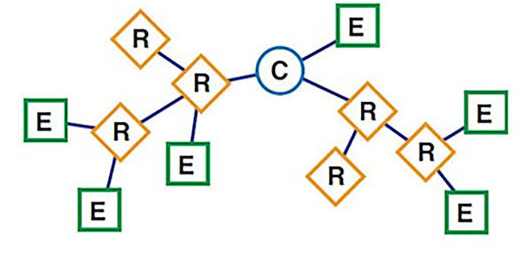
\includegraphics[width=15cm]{images/network}}
  \caption{A Mesh Network of Zigbee Devices}
  \label{fig:quadrotor_trajectory}
\end{figure}	   
	   
	   In the network currently implemented, there are only two nodes. One acting as the coordinator at the ground station and the other acting as an End point near the sensors. We used 802.15.4 protocol to achieve higher point to point transmission speed but this restricts the network to be only a point to point with no possibility of forming meshes of nodes. 

	   
	   